\documentclass[12pt]{report}
\usepackage{graphicx}
\usepackage{setspace}
\usepackage{parskip}
\usepackage{fancyhdr}
\usepackage{titlesec}
\usepackage{lipsum}
\usepackage[margin=1in]{geometry}
\pagestyle{fancy}
\fancyhf{}
\fancyhead[L]{Annual Report}
\fancyhead[R]{\thepage}
\fancyfoot[C]{Confidential}
\renewcommand{\headrulewidth}{0.4pt}
\renewcommand{\footrulewidth}{0pt}
\titleformat{\chapter}[display]{\normalfont\huge\bfseries}{\chaptertitlename\ \thechapter}{20pt}{\Huge}
\onehalfspacing

\begin{document}
\begin{titlepage}
\centering
{\Huge\bfseries Annual Research Report 2024\par}
\vspace{2cm}
{\Large Department of Physics\par}
\vfill
{\large \today\par}
\end{titlepage}

\pagenumbering{roman}
\tableofcontents
\listoffigures
\listoftables
\clearpage
\pagenumbering{arabic}

\chapter{Introduction}\label{ch:intro}
This report summarises the work of the department in 2024. Chapter~\ref{ch:results} presents results.

\section{Background}
\lipsum[1]

\section{Goals}
\begin{itemize}
  \item Increase output.
  \item Improve collaboration.
\end{itemize}

\chapter{Results}\label{ch:results}
\section{Publications}
We published 42 papers.\footnote{Including preprints.}

\begin{figure}[htbp]
  \centering
  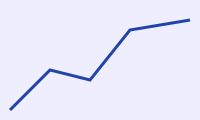
\includegraphics[width=0.6\textwidth]{plot.svg}
  \caption{Publications per month.}
  \label{fig:pubs}
\end{figure}

\begin{table}[H]
\centering
\caption{Funding by source}\label{tab:funding}
\begin{tabular}{lr}
\hline
Source & Amount (k\$) \\
\hline
NSF & 1200 \\
DOE & 800 \\
\hline
\end{tabular}
\end{table}

\chapter*{Acknowledgements}
\addcontentsline{toc}{chapter}{Acknowledgements}
We thank everyone.

\appendix
\chapter{Data}
Raw data are available on request.
\end{document}
